\chapter{Results}\label{chapter:results}

This chapter measures whether a micro-frontend with GraphQL and a shared caching layer can provide a performance improvement for the prototype implementation of the micro-frontend architecture. 

\section{Performance measurement}

Three different approaches were identified to measure the performance of the shared GraphQL caching layer.

\begin{enumerate}
    \item Separate Cache and no reduced queries
    \item Shared Cache and no reduced queries
    \item Shared Cache and reduced queries
\end{enumerate}

To measure the performance of these three approaches, two exemplary paths through the application were created. These examples were intended to show how many network requests were made to the GraphQL backend and how much network traffic was generated.

To make the measurement as close as possible to a real application, a large amount of data was added to the GraphQL backend. With this amount of data, it is easier to measure the difference in response size. The next section details the results of the first path through the application.

\subsection{Evaluation}

The following steps show the first path through the application. 

\begin{enumerate}
    \item Open Dashboard
    \item Open Contacts
    \item Open second Contacts page
    \item Open the first contact on the second page
    \item Open Invoices
    \item Open second Invoices page
    \item Open the first invoice on the second page
    \item Open Contracts
    \item Open second Contracts page
    \item Open the first Contract on the second page
    \item Open Users
    \item Open second Users page
    \item Open the first User on the second page
\end{enumerate}

For the path through the application \textbf{59} GraphQL queries would have to be executed against the backend, if no caching mechanism were in place. The next sections highlight the results in more detail.

To make the testing process easier, I wrote a provider that allows me to easily change the settings to match one of the three approaches. As shown in listing \ref{listing:results:graphql-client-configuration} the UI\_GRAPHQL\_CLIENT\_OPTIONS\_CONFIG injection-token can be used to set if the cache should be should be shared (shareCache) or if a new instance of the cache should be provided. The settings of UI\_REDUCE\_QUERY\_OPTIONS (reduceQueries) can be used, whether the queries should be reduced with the data already inside the cache or not.

\ifshowListings
\begin{listing}[H]
\begin{minted}{typescript}
@NgModule({
  provide: [
    {
      provide: UI_GRAPHQL_CLIENT_OPTIONS_CONFIG,  
      useValue: {  
        shareCache: false,  
        persistCache: false,  
        useTypePolicies: true,  
        typePolicies: UI_DASHBOARD_APP_TYPE_POLICIES,  
      } as UiGraphQLClientOptionsConfig,  
    },  
    {  
      provide: UI_REDUCE_QUERY_OPTIONS,  
      useValue: {  
        reduceQueries: false,  
      } as UiReduceQueryOptions,  
    }
   ],
})
export class UiContactRemoteCoreModule {}
\end{minted}
\caption{Providers to configure the behavior of the cache and query-reduction}\label{listing:results:graphql-client-configuration}
\end{listing}
\fi

\begin{itemize}
    \item allEmailTypes: 1
    \item allSalutations: 5
    \item allContactsSubset: 1
    \item contactTitlesAggregated: 1
    \item allTitles: 5
    \item allContractsSubset: 1
    \item allInvoicesSubset: 1
    \item contactCountriesAggregated: 1
    \item allCountries: 5
    \item allArticleUnits: 3
    \item allCurrencies: 3
    \item allVats: 3
    \item allSalesCountries: 5
    \item allInvoiceTypes: 3
    \item allUsersSubset: 1
    \item \_allContactsMeta: 2
    \item allContacts: 2
    \item Contact: 1
    \item \_allInvoicesMeta: 2
    \item allInvoices: 2
    \item Invoice: 1
    \item \_allContractsMeta: 2
    \item allContracts: 2
    \item Contract: 1
    \item \_allUsersMeta: 2
    \item allUsers: 2
    \item User: 1
\end{itemize}

\subsubsection{Separate cache, no query reduction}

In this approach, each micro frontend has its own instance of the GraphQL client and cache. The queries are not reduced using the cache.

After completing the path through the applications, the Chrome Developer Tools provide the following metrics:

\begin{itemize}
    \item 47 GraphQL requests
    \item 10.7 MB transferred
\end{itemize}

 To configure this behavior the following settings have to be provided to the UI\_GRAPHQL\_CLIENT\_OPTIONS\_CONFIG- and UI\_REDUCE\_QUERY\_OPTIONS injection-tokens inside the core-modules of the micro-frontend.

\begin{itemize}
    \item shareCache: false
    \item reduceQueries: false
\end{itemize}

47 requests have to be made to the GraphQL backend which can be seen in figure \ref{figure:results:no-shared-cache-no-reduction-chrome-dev-tools}. 6 of the 53 requests have to be removed, because these requests are done to load the other micro-frontends from their remote location. These requests are only needed for the functionality of the micro-service architecture.

\ifshowImages
\begin{figure}[H]
\centering
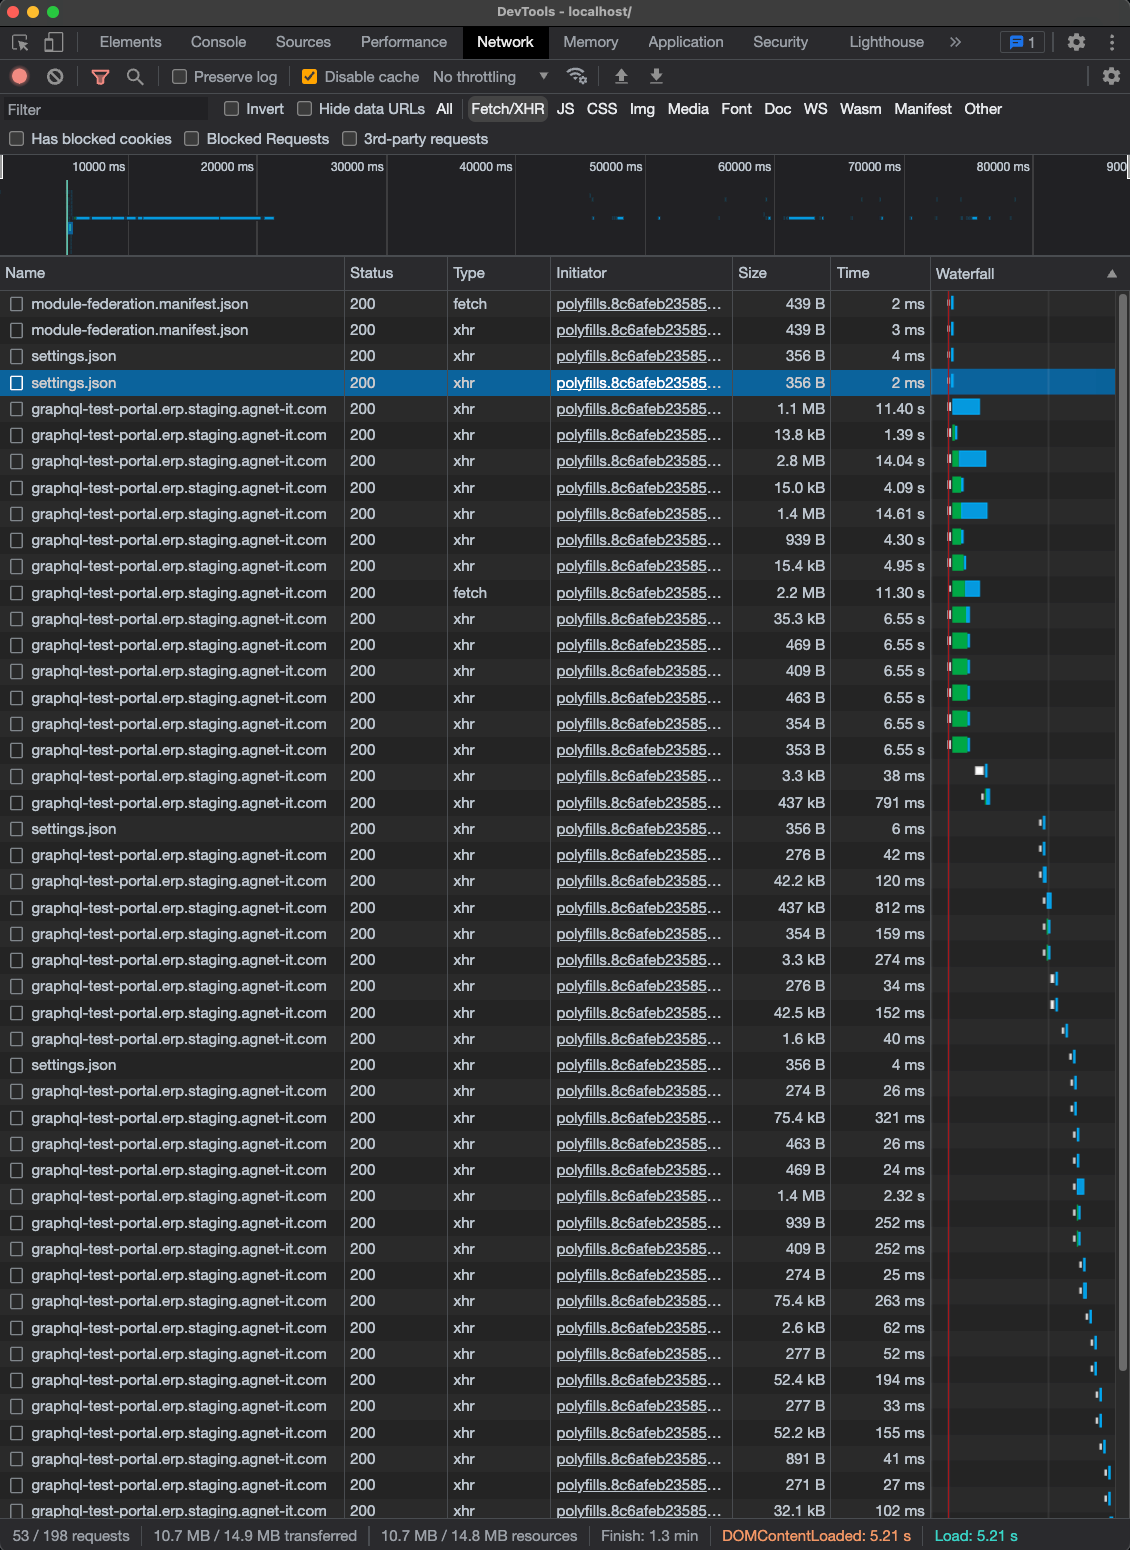
\includegraphics[width=0.6\linewidth]{images/1-attempt/no-shared-cache-no-reduction.png}
\caption{All requests made during the measurement of the first approach}\label{figure:results:no-shared-cache-no-reduction-chrome-dev-tools}
\end{figure}
\fi

The total size of the queries was 17.46 KB and the size of the responses was 10.78 MB. The 47 queries retrieve a total of 61426 records from the GraphQL backend.

\subsubsection{Shared cache, no query reduction}

In this approach, the cache is shared by all micro-frontends and queries are not reduced by data already present in the cache.

After completing the path, the Chrome Developer Tools provide the following metrics:

\begin{itemize}
    \item 36 GraphQL requests
    \item 8.5 MB transferred
\end{itemize}

 To configure this behavior the following settings have to be provided to the UI\_GRAPHQL\_CLIENT\_OPTIONS\_CONFIG- and UI\_REDUCE\_QUERY\_OPTIONS injection-tokens inside the core-modules of the micro-frontends.

\begin{itemize}
    \item shareCache: true
    \item reduceQueries: false
\end{itemize}

36 requests have to be made to the GraphQL backend which can be seen in figure \ref{figure:results:no-shared-cache-no-reduction-chrome-dev-tools}. 6 requests have to be subtracted (settings.json, module-federation.manifest.json) like previously.

\ifshowImages
\begin{figure}[H]
\centering
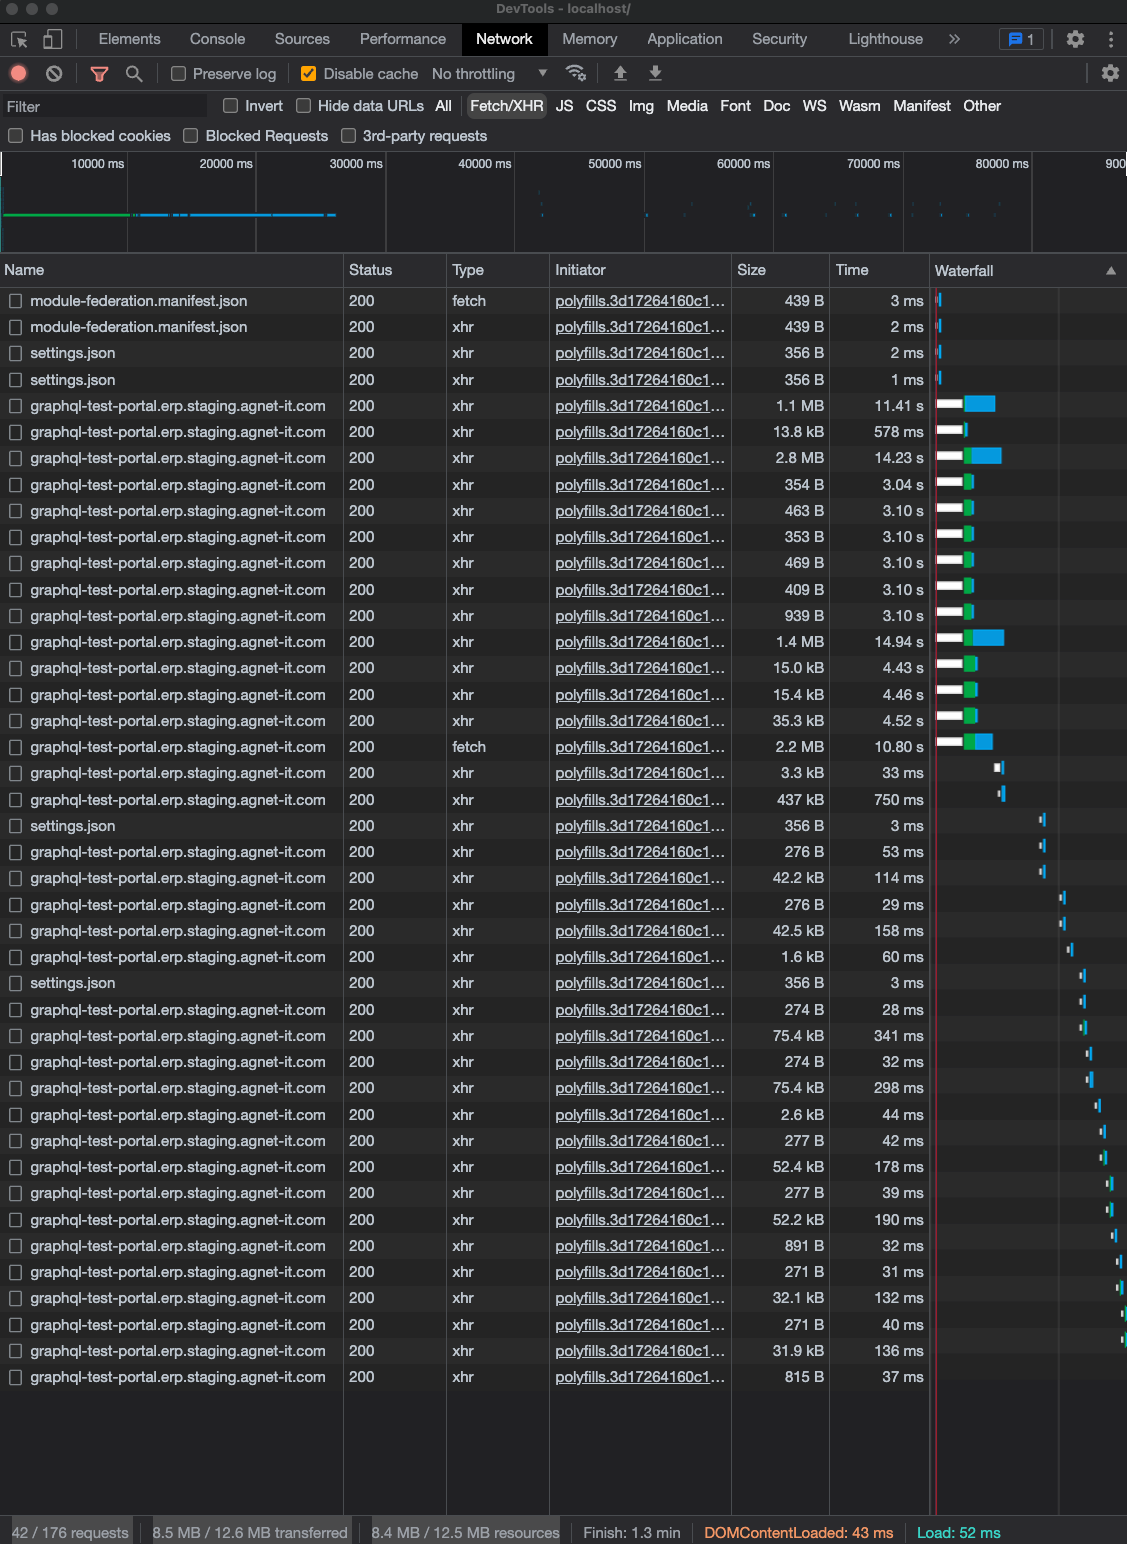
\includegraphics[width=0.6\linewidth]{images/1-attempt/shared-not-reduced-cache.png}
\caption{All requests made during the measurement of the second approach}\label{figure:results:shared-cache-no-reduction-chrome-dev-tools}
\end{figure}
\fi

The total size of the queries was 15.176 KB and the size of the responses was 8.5 MB. The 36 queries retrieve a total of 51319 records from the GraphQL backend.

\subsubsection{Shared cache, query reduction}

With this approach, the cache is shared between all the micro-frontends and the queries are reduced with already existing data inside the cache.

After completing the path, the Chrome Developer Tools provide the following metrics:

\begin{itemize}
    \item 36 GraphQL requests
    \item 8.4 MB transferred
\end{itemize}

 To configure this behavior the following settings have to be provided to the UI\_GRAPHQL\_CLIENT\_OPTIONS\_CONFIG- and UI\_REDUCE\_QUERY\_OPTIONS injection-tokens inside the core-modules of the micro-frontends.

\begin{itemize}
    \item shareCache: true
    \item reduceQueries: false
\end{itemize}

36 requests have to be made to the GraphQL backend which can be seen in figure \ref{figure:results:no-shared-cache-no-reduction-chrome-dev-tools}. 6 requests have to be subtracted (settings.json, module-federation.manifest.json).

\ifshowImages
\begin{figure}[H]
\centering
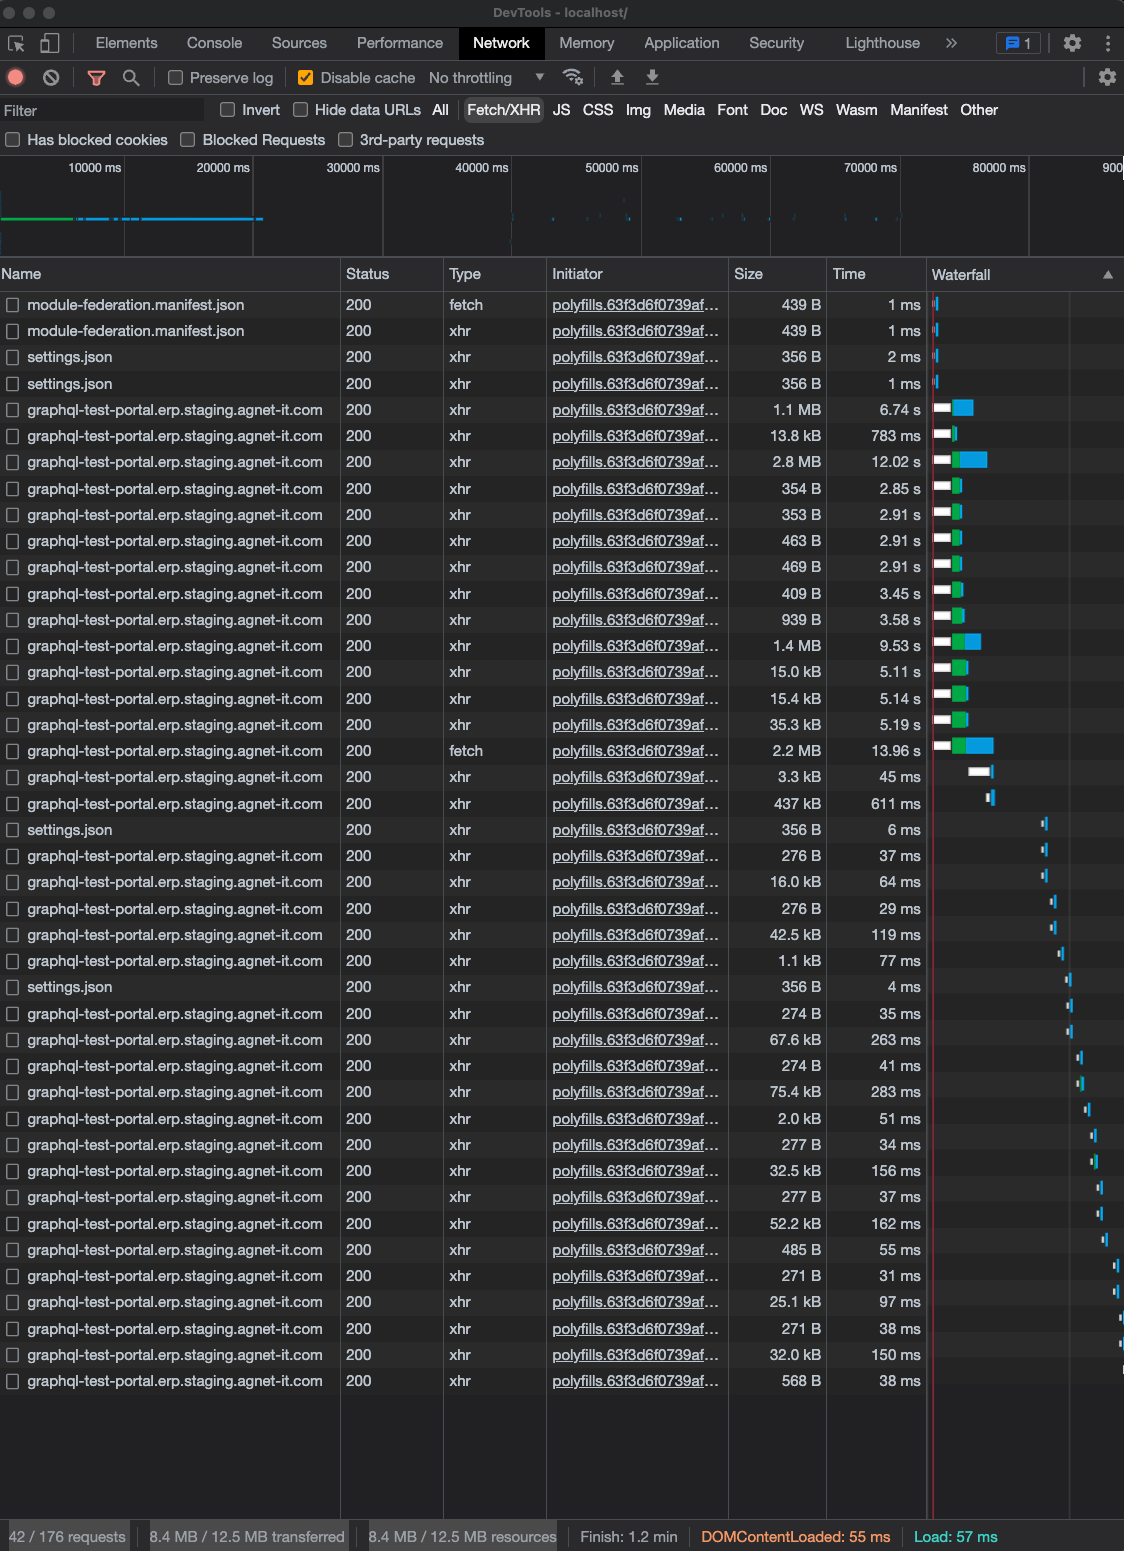
\includegraphics[width=0.6\linewidth]{images/1-attempt/shared-reduced-cache.png}
\caption{All requests made during the measurement of the third approach}\label{figure:results:shared-cache-reduction-chrome-dev-tools}
\end{figure}
\fi

The total size of the queries was 13.533 KB and the size of the responses was 8.37 MB. The 36 queries retrieve a total of 51319 records from the GraphQL backend.

\subsubsection{Comparison between the three approaches}

This section compares compares the different approaches in terms of request- and response-size.

\paragraph{Comparing the first- and second-approach}

When comparing the first- with the second-approach there is a massive difference in the amount of network-requests made to the GraphQL backend and the size of the requests and responses, as seen in table \ref{table:results:size-comparison-first-path-no-cache-no-reduction-cache-no-reduction}. The shared cache approach requires 11 fewer network requests than the separate cache approach. Since the queries are not reduced in this comparison, the additional network queries account for the overall difference in request- and response-size. The 11 additional requests from the first approach send an additional 2.29 KB to the backend and return about an additional 2.34 MB from the backend. Therefore, 22\% of the total response-size can be saved by using only one shared cache. Another interesting observation is that the shared cache approach retrieves 10107 fewer records than the naive approach, which is 16\% of the total records returned.

\ifshowTables
\begin{table}[H]
    \begin{tabular}{|l|l|l|l|l|}
    \hline
      & Request Size (B) & Response Size (B) & Requests & Records \\
    \hline
     No Reduction, Separate Cache & 17462 & 10780656 & 47 & 61426 \\
     \hline
     No Reduction, Shared Cache & 15176 & 8437211 & 36 & 51319 \\
     \hline
     \hline
     \textbf{Diff} & \textbf{2286} & \textbf{2343445} & \textbf{11} & \textbf{10107} \\
     \hline
     \textbf{Reduction \%} & \textbf{13\%} & \textbf{22\%} & \textbf{23\%} & \textbf{16\%} \\
     \hline
    \end{tabular}
    \caption{Comparing the requests and responses of the first- and second-approach.}
    \label{table:results:size-comparison-first-path-no-cache-no-reduction-cache-no-reduction}
\end{table}
\fi

Following requests have been omitted, when using a shared cache between the micro-frontends:

\begin{itemize}
    \item allCountries(User-MF, Contact-MF): 2
    \item allSalutations(User-MF, Contact-MF): 2
    \item allTitles(User-MF, Contact-MF): 2
    \item allArticleUnits(Sales-MF): 1
    \item allCurrencies(Sales-MF): 1
    \item allVats(Sales-MF): 1
    \item allSalesCountries(Sales-MF): 1
    \item allInvoiceTypes(Sales-MF): 1
\end{itemize}

The data of the requests is usually used for filling select-controls inside detail-views and has to be fetched in every micro-frontends, when not using a shared-cache. The first three queries are used inside micro-frontends on the dashboard, the contact micro-frontend and the user micro-frontend. The last five queries are used inside micro-frontends on the dashboard and the sales micro-frontend.

\paragraph{Comparing the first- and third-approach}

Like in the previous comparison, there is also a massive difference in the amount of network-requests made to the GraphQL backend and the size of the requests and responses, as seen in table \ref{table:results:size-comparison-first-path-no-cache-no-reduction-cache-reduction}. Just like before, there is a difference in the 11 GraphQL queries that are sent to the backend. However, due to the reduction in queries, the difference in the size of the queries and responses is greater than before. All queries of the first approach send 3.92 KB more and return about 2.41 MB more from the backend compared to the third approach. A shared cache and query reduction can save about 22\% response size. As before, 16\% fewer records need to be fetched from the backend.

\ifshowTables
\begin{table}[H]
    \begin{tabular}{|l|l|l|l|l|}
    \hline
       & Request Size (B) & Response Size (B) & Requests & Records  \\
    \hline
     No Reduction, Separate Cache & 17462 & 10780656 & 47 & 61426 \\
     \hline
     Reduction, Shared Cache & 13533 & 8374763 & 36 & 51319 \\
     \hline
     \hline
     \textbf{Diff} & \textbf{3929} & \textbf{2405893} & \textbf{11} & \textbf{10107} \\
     \hline
    \textbf{Reduction \%} & \textbf{23\%} & \textbf{22\%} & \textbf{23\%} & \textbf{16\%} \\
     \hline
    \end{tabular}
    \caption{Comparing the requests and responses of the first- and third-approach.}
    \label{table:results:size-comparison-first-path-no-cache-no-reduction-cache-reduction}
\end{table}
\fi

\paragraph{Comparing the second- and third-approach}

Between the first- and the second-approach, there is almost no difference in request- and response-size compared to the other comparisons, as seen in table \ref{table:results:size-comparison-first-path-no-cache-no-reduction-cache-reduction}. As seen earlier, both approaches have the same number of queries since the cache is shared by all micro-frontends. Thus, the only difference in request and response size between the two approaches comes from the use of query reduction. By using the third approach, the size of the total requests is reduced by 1.64 KB (11\%). The difference between the response sizes (62.45 KB) is almost zero compared to the amount of data returned.

\ifshowTables
\begin{table}[H]
    \begin{tabular}{|l|l|l|l|l|}
    \hline
      & Request Size (B) & Response Size (B) & Requests & Records \\
    \hline
     No Reduction, Shared Cache & 15176 &  8437211 & 36 & 51319 \\
     \hline
     Reduction, Shared Cache &  13533 &  8374763 & 36 & 51319 \\
     \hline
     \hline
     \textbf{Diff} & \textbf{1643} & \textbf{62448} & \textbf{0} & \textbf{0} \\
     \hline
     \textbf{Reduction \%} & \textbf{11\%} & \textbf{0\%} & \textbf{-} & \textbf{-} \\
     \hline
    \end{tabular}
    \caption{Comparing the requests and responses of the second- and third-approach.}
    \label{table:results:size-comparison-first-path-cache-no-reduction-cache-reduction}
\end{table}
\fi

\subsection{2. Attempt}

The following enumeration shows the second path through the application. This attempt was made, with an authenticated user.

\begin{enumerate}
    \item Open Users
    \item Open second Users page
    \item Open the first User on the second page
    \item Open the second User on the second page
    \item Open Invoices
    \item Open second Invoices page
    \item Open the first invoice on the second page
    \item Open the second invoice on the second page
    \item Open Contracts
    \item Open second Contracts page
    \item Open the first Contract on the second page
    \item Open the second Contract on the second page
    \item Open Contacts
    \item Open second Contacts page
    \item Open the first Contact on the second page
    \item Open the second Contact on the second page
    \item Open Dashboard
\end{enumerate}

For this path through the application \textbf{59} queries in total have to be executed against the
GraphQL backend, when no caching mechanism are implemented.

\begin{itemize}
    \item userByToken: 9
    \item \_allUsersMeta: 2
    \item allUsers: 2
    \item allCountries: 5
    \item allSalutations: 5
    \item allTitles: 5
    \item User: 2
    \item \_allInvoicesMeta: 2
    \item allInvoices: 2
    \item allArticleUnits: 3
    \item allCurrencies: 3
    \item allVats: 3
    \item allSalesCountries: 5
    \item allInvoiceTypes: 3
    \item Invoice: 2
    \item \_allContractsMeta: 2
    \item allContracts: 2
    \item Contract: 2
    \item \_allContactsMeta: 2
    \item allContacts: 2
    \item Contact: 2
    \item allEmailTypes: 1
    \item allContactsSubset: 1
    \item contactTitlesAggregated: 1
    \item allContractsSubset: 1
    \item allInvoicesSubset: 1
    \item contactCountriesAggregated: 1
    \item allUsersSubset: 1
\end{itemize}

\begin{table}[]
    \begin{tabular}{|l|l|l|l|}
    \hline
                                    & Request Size & Response Size & Request Amount  \\
    \hline
     No Reduction, Shared Cache     &  16884 B        &  8364416 B   & 37 \\
     \hline
     Reduction, Shared Cache        &  14718 B        &  8361306 B   & 37 \\
     \hline
    \textbf{Diff}                   & \textbf{2166 B (0.0016 MB)} & \textbf{3110 B (0.062  MB)} & \textbf{11} \\
     \hline
    \end{tabular}
    \caption{Vergleich der State of the art Serious games.}
    \label{tab:serious-game-comparison}
\end{table}

\begin{table}[]
    \begin{tabular}{|l|l|l|l|}
    \hline
                                    & Request Size & Response Size & Request Amount  \\
    \hline
     No Reduction, No Shared Cache     &  22955 B        &  10713304 B   & 62 \\
     \hline
     Reduction, Shared Cache        &  14718 B        &  8361306 B   & 37 \\
     \hline
    \textbf{Diff}                   & \textbf{8237 B (0.0016 MB)} & \textbf{2351998 B (0.062  MB)} & \textbf{25} \\
     \hline
    \end{tabular}
    \caption{Vergleich der State of the art Serious games.}
    \label{tab:serious-game-comparison}
\end{table}

\begin{table}[]
    \begin{tabular}{|l|l|l|l|}
    \hline
                                    & Request Size & Response Size & Request Amount  \\
    \hline
     No Reduction, No Shared Cache     &  22955 B        &  10713304 B   & 62 \\
     \hline
     No Reduction, Shared Cache        &  16884 B        &  8364416 B   & 37 \\
     \hline
    \textbf{Diff}                   & \textbf{6071 B (0.0016 MB)} & \textbf{2348888 B (0.062  MB)} & \textbf{25} \\
     \hline
    \end{tabular}
    \caption{Vergleich der State of the art Serious games.}
    \label{tab:serious-game-comparison}
\end{table}

% \section{Stale data}

